% \ano{corrected t test p/ avaliar 2 algs em 1 dataset; wilcoxon em vários}
As escolhas metodológicas expostas neste capítulo fundamentam a avaliação experimental das propostas deste trabalho.
% para identificar os pontos críticos na escolha de estratégias e também para comprovação empírica.
Na Seção \ref{desccen}, são apresentados detalhes sobre o cenário adotado.
Os conjuntos de dados, utilizados visando a simulação de aplicações reais, são descritos e analisados sob diferentes aspectos na Seção \ref{desccon}.
Nas seções \ref{learners} e \ref{confstrats}, os parâmetros são definidos e considerações são feitas sobre as estratégias de amostragem ativa e os algoritmos de aprendizado empregados - respectivamente.
As medidas de desempenho, a forma de validação e o tipo de teste empregado para a avaliação da significância estatística dos resultados experimentais são apresentados na Seção \ref{avaliacao}.
Na Seção \ref{sec:curvas}, são introduzidas as curvas de ranqueamento - importante contribuição metodológica deste trabalho.
Por fim, a Seção \ref{sec:consider} contém as considerações gerais.
\usetikzlibrary{trees}

Parte das decisões tomadas foram baseadas num experimento preliminar.
Ele permitiu a definição de experimentos definitivos adequados aos recursos computacionais disponíveis.
% Nesse teste inicial, dez estratégias de aprendizado ativo
% % (C4.5, NB, VFDT e 5-NN)
% foram comparadas.
% Dez execuções de validação cruzada em dez partições totalizaram 100 \pools para cada conjunto - conforme sugerido por \citeonline{conf/pakdd/BouckaertF04}.
% As \pools foram consultadas até o ponto em que a acurácia máxima da melhor estratégia fosse atingida.
Aproximadamente um mês foi necessário para a conclusão do experimento nos 28 menores conjuntos de dados.
Assim, considerando-se o crescimento exponencial do custo computacional em alguns pares estratégia-algoritmo com o aumento do número de classes, atributos e/ou exemplos, foi necessário reduzir a quantidade de iterações do procedimento de validação e antecipar o término das consultas.
Os resultados desse experimento preliminar com relação a desempenho não são reportados nesta tese por serem menos abrangentes que o experimento definitivo.
Mais detalhes podem ser encontrados em \citeonline{conf/hais/SantosC14}.

\section{Cenário escolhido}\label{desccen}
É necessário situar o escopo do presente trabalho, dado o grande número de possibilidades dentro dos cenários e restrições que possam existir num dado problema.
Existem três principais cenários na literatura de aprendizado ativo
\cite{settles2010active}:
\textit{síntese de consulta por associação} ou
\ing{consulta de exemplos sintetizados}{membership query synthesis};
\textit{amostragem baseada em \pool}; e,
\textit{amostragem seletiva baseada em fluxo}.
% Mais detalhes são apresentados no Apêndice \ref{cenarios}.
O cenário adotado neste trabalho é baseado em \pool.
Especificamente, há as seguintes restrições de escopo:
\begin{itemize}
 \item problemas monorrótulo multiclasse;
 \item consulta pela classe (não por valores de atributos, por exemplo);
 \item conjunto ou quantidade de classes possíveis previamente conhecida;
 \item distribuição das classes não necessariamente balanceada;
 \item distribuição estacionária;
 \item custo por erro de classificação uniforme;
 \item custo por consulta uniforme;
 \item oráculo único e sujeito a ruído consistente (sempre comete os mesmos erros);
 \item os domínios dos atributos nominais são previamente conhecidos;
 \item atributos sem valores faltantes; e,
 \item consulta \textit{on-line}, ou seja, um a um.
\end{itemize}
As seguintes condições foram criadas visando maior rigor experimental, replicabilidade e verossimilhança com aplicações reais:
\begin{itemize}
 \item um rótulo inicial por classe;
 \item todo o conjunto de dados original é utilizado no processo de validação cruzada - exceto exemplos duplicados e no caso de EER (Seção \ref{eerconfig}); e,
 \item critério de parada determinado pelo orçamento de cem consultas ($\cent=100$).
 \end{itemize}
Uma condição mínima necessária a diversas estratégias é existir, no modelo de classificação, a capacidade de estimar pelo menos um esboço da fronteira de decisão - vide critérios de consulta no Capítulo \ref{contexto}.
Consequentemente, optou-se pela adoção de um exemplo rotulado inicial por classe.
Além dessa ser a quantidade mínima para que um modelo seja induzido e possa estimar uma fronteira de decisão, ela também reflete a cautela necessária em aplicações reais, pois o aprendizado ativo não garante que exemplos de todas as classes sejam consultados.
Por exemplo, quanto maior o grau de desbalanceamento entre as classes, maior o custo com consultas adicionais necessárias até que todas as classes sejam contempladas.
Portanto, é importante obter criteriosamente alguns rótulos antes de ser iniciado o processo de amostragem ativa.

Uma maneira de obter um rótulo por classe é por meio do \textit{aprendizado guiado} \cite{conf/kdd/AttenbergP10}.
Esse tipo de aprendizado realiza uma amostragem em que o usuário escolhe os exemplos a rotular.
Normalmente, ele sabe de antemão as classes menos frequentes e é capaz de encontrar exemplos correspondentes, seja por meio de consulta a motores de busca na \textit{internet}, da própria memória pessoal ou de outras formas.
Essa modalidade de amostragem faz maior usufruto da capacidade da inteligência humana enquanto agente supervisor do que a simples rotulação.
Embora custoso, esse potencial humano pode ser aproveitado no estágio inicial da rotulação e favorecer a posterior amostragem ativa, minimizando as futuras intervenções humanas.

A prática de rotulação prévia em experimentos também tem sido parte da metodologia adotada em outros trabalhos \cite{conf/nips/GuoS07, conf/cvpr/BiswasP13, conf/iconip/GuJC14a}, com variações mais permissivas com relação à quantidade de exemplos \cite{journals/prl/PatraB12} ou substituída por uma amostragem aleatória aplicada até que se encontre um exemplo de cada classe \cite{chermanaprendizado}.

A limitação a um número fixo de consultas segue a observação de \citeonline{series/synthesis/2012Settles} sobre o critério desejável de parada do processo de aprendizado ativo. 
Ele relata que, em aplicações reais, normalmente trata-se de uma restrição financeira.
Consequentemente, a definição do orçamento para fins experimentais tem sido arbitrária na literatura, sendo 100 consultas um valor recorrente \cite{journals/pieee/CrawfordTY13,chermanaprendizado,conf/nips/SettlesCR07,conf/icml/RoyM01,conf/emnlp/SettlesC08}.
 
Outra característica presente nos experimentos está no não aproveitamento da informação de orçamento disponível - decisão usual na literatura \cite{conf/icml/RoyM01}.
Isso implica na geração de sequências de consultas provavelmente não ótimas, ou, em outras palavras, cada consulta é realizada como se fosse a última.
Uma consulta ótima dependeria de quantas ainda poderiam ser feitas.
Apesar de ser uma possibilidade teórica, seu não aproveitamento não é uma limitação real, pois não é esperado que existam estratégias capazes de tirar proveito dessa informação de forma significativa.

\section{Conjuntos de dados}\label{desccon}
Os conjuntos de dados do projeto de \citeonline{doi/ucipp}, baseado no repositório da \sigla{UCI}{Universidade da Califórnia, Irvine} - \cite{bache2013uci}, foram utilizados com o objetivo de representar os variados domínios existentes em aplicações reais.
Parte dos conjuntos foi descartada conforme descrito nas seções \ref{sectempo} e \ref{secsimi}.
Os critérios de descarte objetivaram selecionar os conjuntos mais adequados\footnote{Análises posteriores à primeira versão deste documento demonstraram uma importante deficiência na coleção adotada (Apêndice \ref{apflu}).} para a coleção utilizada nos experimentos desta tese.
Contudo, a análise dos experimentos leva em conta que o propósito da construção de uma coleção representativa de conjuntos de dados não é a demonstração da superioridade de algum algoritmo em todos os casos, mas identificar os pontos fortes de cada algoritmo  \cite{books/cu/Japkowicz2011}.
% The purpose of data set selection should not be to demonstrate an algorithm’s superiority to another in all cases, but rather to identify the areas of strengths of various algorithms with respect to domain characteristics or on specific domains of interest.

\subsection{Custo computacional}\label{sectempo}
Dada a quantidade envolvida de estratégias de amostragem ativa, algoritmos de aprendizado e execuções de validação por conjunto de dados (Seção \ref{validacao}), a limitação do tempo de processamento foi essencial para que os experimentos previstos fossem realizados.
Essa limitação não afetou os experimentos, pois o foco é a acurácia preditiva.
Logo, os conjuntos de dados que demandam excessivo tempo para a inicialização de estratégias ou para a realização de consultas foram descartados, permitindo a viabilidade computacional dos experimentos.
Esse tempo foi estimado por meio de um experimento reduzido.
Ele consistiu na execução de validação cruzada em duas partes aplicada apenas ao algoritmo com maior custo computacional (RoF - Seção \ref{learners}) e três estratégias, cada uma com sua respectiva particularidade referente ao custo computacional:
\begin{itemize}
   \item ATU - inicialização requer quantidade quadrática de cálculos de distância em relação ao tamanho da reserva de exemplos;
   \item SGmulti - consulta requer quantidade de treinamentos proporcional ao número de classes; e,
   \item EER - consulta requer quantidade de treinamentos proporcional ao número de classes e quadrática com relação ao número de exemplos.
\end{itemize}
Os seguintes conjuntos de dados foram descartados, uma vez que atingiram um tempo de processamento entre 4 e 16 horas para as primeiras 50 consultas no experimento reduzido:
% +ou- ordenado por tempo
\textit{arcene, micro mass pure spectra, micro mass mixed spectra, multiple features, digits2, lsvt voice rehabilitation, semeion, cnae 9, gas drift, gas drift different concentrations} e \textit{hill valley with noise}.
Estimou-se um tempo entre 700 e 2800 dias para cada um desses conjuntos no experimento definitivo, tomando por base as seguintes considerações:
\begin{itemize}
   \item 100 consultas contêm 3 vezes mais unidades de treinamento\footnote{Quantidade de exemplos de treinamento. Todos são reaprendidos a cada nova consulta.} que 50 consultas;
   \item seriam avaliados, no pior caso, 8 algoritmos e 14 estratégias; e,
   \item o processo de validação consistiria de 25 execuções.
\end{itemize}
Mesmo dividindo esses valores estimados de duração do experimento definitivo pelo número de núcleos de processamento inicialmente disponíveis, 100, não seria viável incluir tais conjuntos de dados.

\subsection{Similaridade}\label{secsimi}
Conjuntos de dados equivalentes ou muito similares foram excluídos dos experimentos desta tese com a finalidade de aumentar a \textit{independência entre amostras} para o teste estatístico (seções \ref{testestbase} e \ref{testestmeta}).
A ausência de redundância entre os conjuntos também é importante para a avaliação adequada da capacidade de generalização do meta-aprendizado: tal como no nível base, metaexemplos não devem aparecer simultaneamente nos conjuntos de teste e treinamento.
A similaridade entre conjuntos foi indiretamente estimada do ponto de vista do viés de aprendizado.
Trata-se de uma escolha conservadora, pois os mesmos vieses podem ser adequados a problemas distintos.
Essa abordagem é baseada na tabela de distâncias entre taxas de erro empregada por \citeonline{brazdil1994analysis}.
Neste trabalho, entretanto, optou-se pela comparação de desempenhos relativos, feita por uma medida de correlação, pois ela proporciona a análise de um ponto de vista mais amplo, independente de valores absolutos de acurácia, por exemplo.
% Brazdil faz tabela de distâncias pareadas com taxas de erro sendo
% as dimensões, depois faz decomposição ortogonal para visualizar em duas dimensões.
% Depois ele faz agrupamento hierárquico.

A correlação de Spearman \cite{reference/stat/GibbonsC11} foi calculada entre os ranqueamentos médios de desempenho de 10 algoritmos de aprendizado (Seção \ref{learners}) com o objetivo de estimar indiretamente a similaridade entre cada par de conjuntos.
A medida de desempenho adotada, $\kappa$ (Seção \ref{newhtu}), foi obtida em 100 execuções de validação cruzada em dez partes.
Valores elevados de correlação foram obtidos devido à frequente superioridade de alguns algoritmos sobre outros  \cite{journals/jmlr/DelgadoCBA14}.
Valores acima de $0,95$ foram considerados indicativos de similaridade excessiva.
Esse foi o maior valor atingido por conjuntos de domínios conhecidamente distintos.

Apenas um conjunto dentre cada grupo de conjuntos similares permaneceu e os demais foram descartados.
Os conjuntos descartados são listados a seguir:
\textit{thyroid allrep, thyroid allhyper, thyroid allhypo, thyroid allbp, thyroid dis, robot failure lp4, leukemia haslinger, robot nav sensor readings 4, cardiotocography 10class, nursery 4class, movement libras 10, mushroom expanded, waveform v1, connectionist vowel reduced, breast tissue 6class, yeast, wine quality 5class, abalone 11class, robot nav sensor readings 24} e variações dos conjuntos \textit{volcanoes} \textit{a}, \textit{b}, \textit{d} e \textit{e}.
Conjuntos em que todos os algoritmos obtiveram um desempenho próximo ao acaso ($\kappa < 0,02$) poderiam gerar colocações de ranqueamento de pares estratégia-algoritmo espúrias, afetando os resultados sem trazer qualquer benefício para os experimentos.
Consequentemente, eles também foram descartados: \textit{autoUniv-au6-1000, autoUniv-au6-1000, autoUniv-au6-250-drift-au6-cd1-500, meta-data, planning-relax} e \textit{monks2}.

A Figura \ref{datasetsimistodos} contém o mapa de calor \cite{wilkinson2009history} que atribui uma intensidade de correlação a cada par dentre os 90 conjuntos de dados que restaram ao fim do processo de descarte.
Este e os demais mapas de calor neste texto estão com as linhas ordenadas pela soma dos valores nas colunas.
O azul e o vermelho mais intensos indicam, respectivamente, o melhor e o pior valor.
A cor branca indica o valor central.
No presente caso, o melhor valor é o mais baixo; em valores de acurácia, distância e correlação na predição de ranqueamentos, o melhor valor é o mais elevado. 
\begin{figure}
  \setlength{\unitlength}{1.0cm}
  \centering
    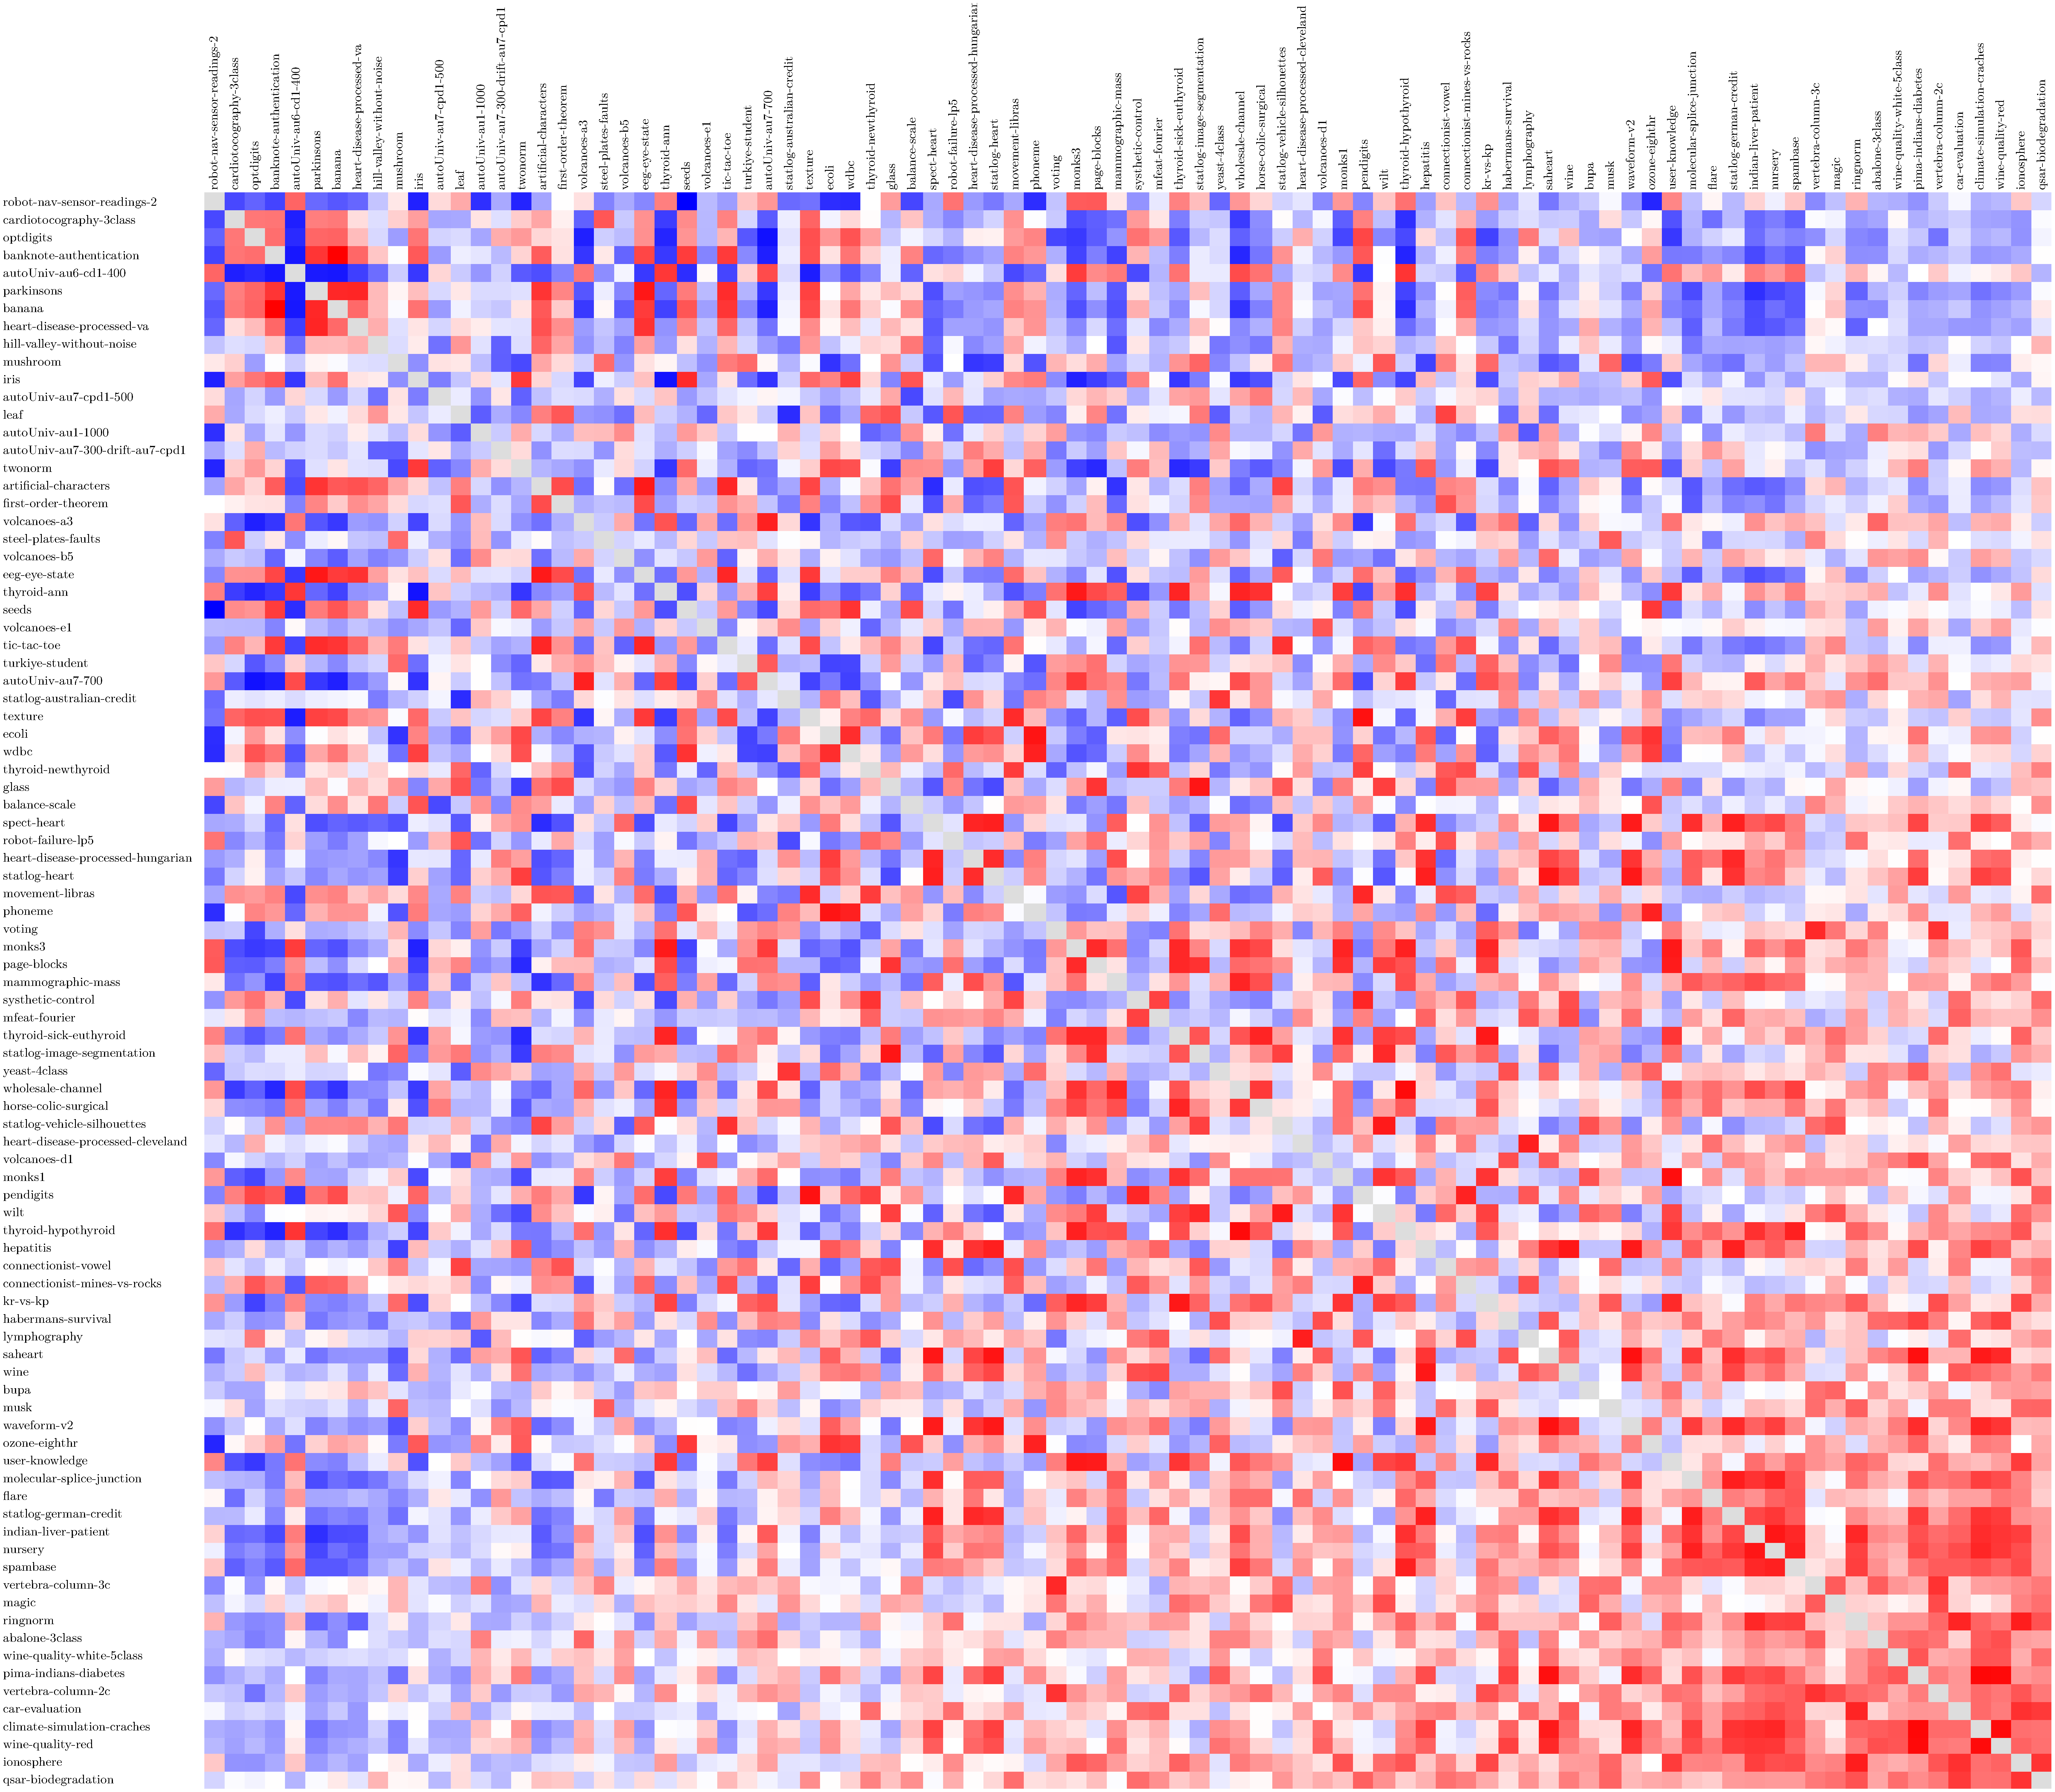
\includegraphics[scale=0.136]{images/heatbitmap.pdf}
  \caption[Correlação entre ranqueamentos de algoritmos de aprendizado.]{Visão geral da intensidade de correlação entre ranqueamentos de algoritmos de aprendizado para cada par possível na coleção. \textit{Azul: mais adequado. Vermelho: menos adequado.}}
  \label{datasetsimistodos}
\end{figure}
O mapa de calor com os valores de correlação dos conjuntos que apresentaram valores acima de $0,8$ é apresentado com maior clareza na Figura \ref{datasetsimis}.
\begin{landscape}
\begin{figure}
  \setlength{\unitlength}{1.0cm}
  \centering
    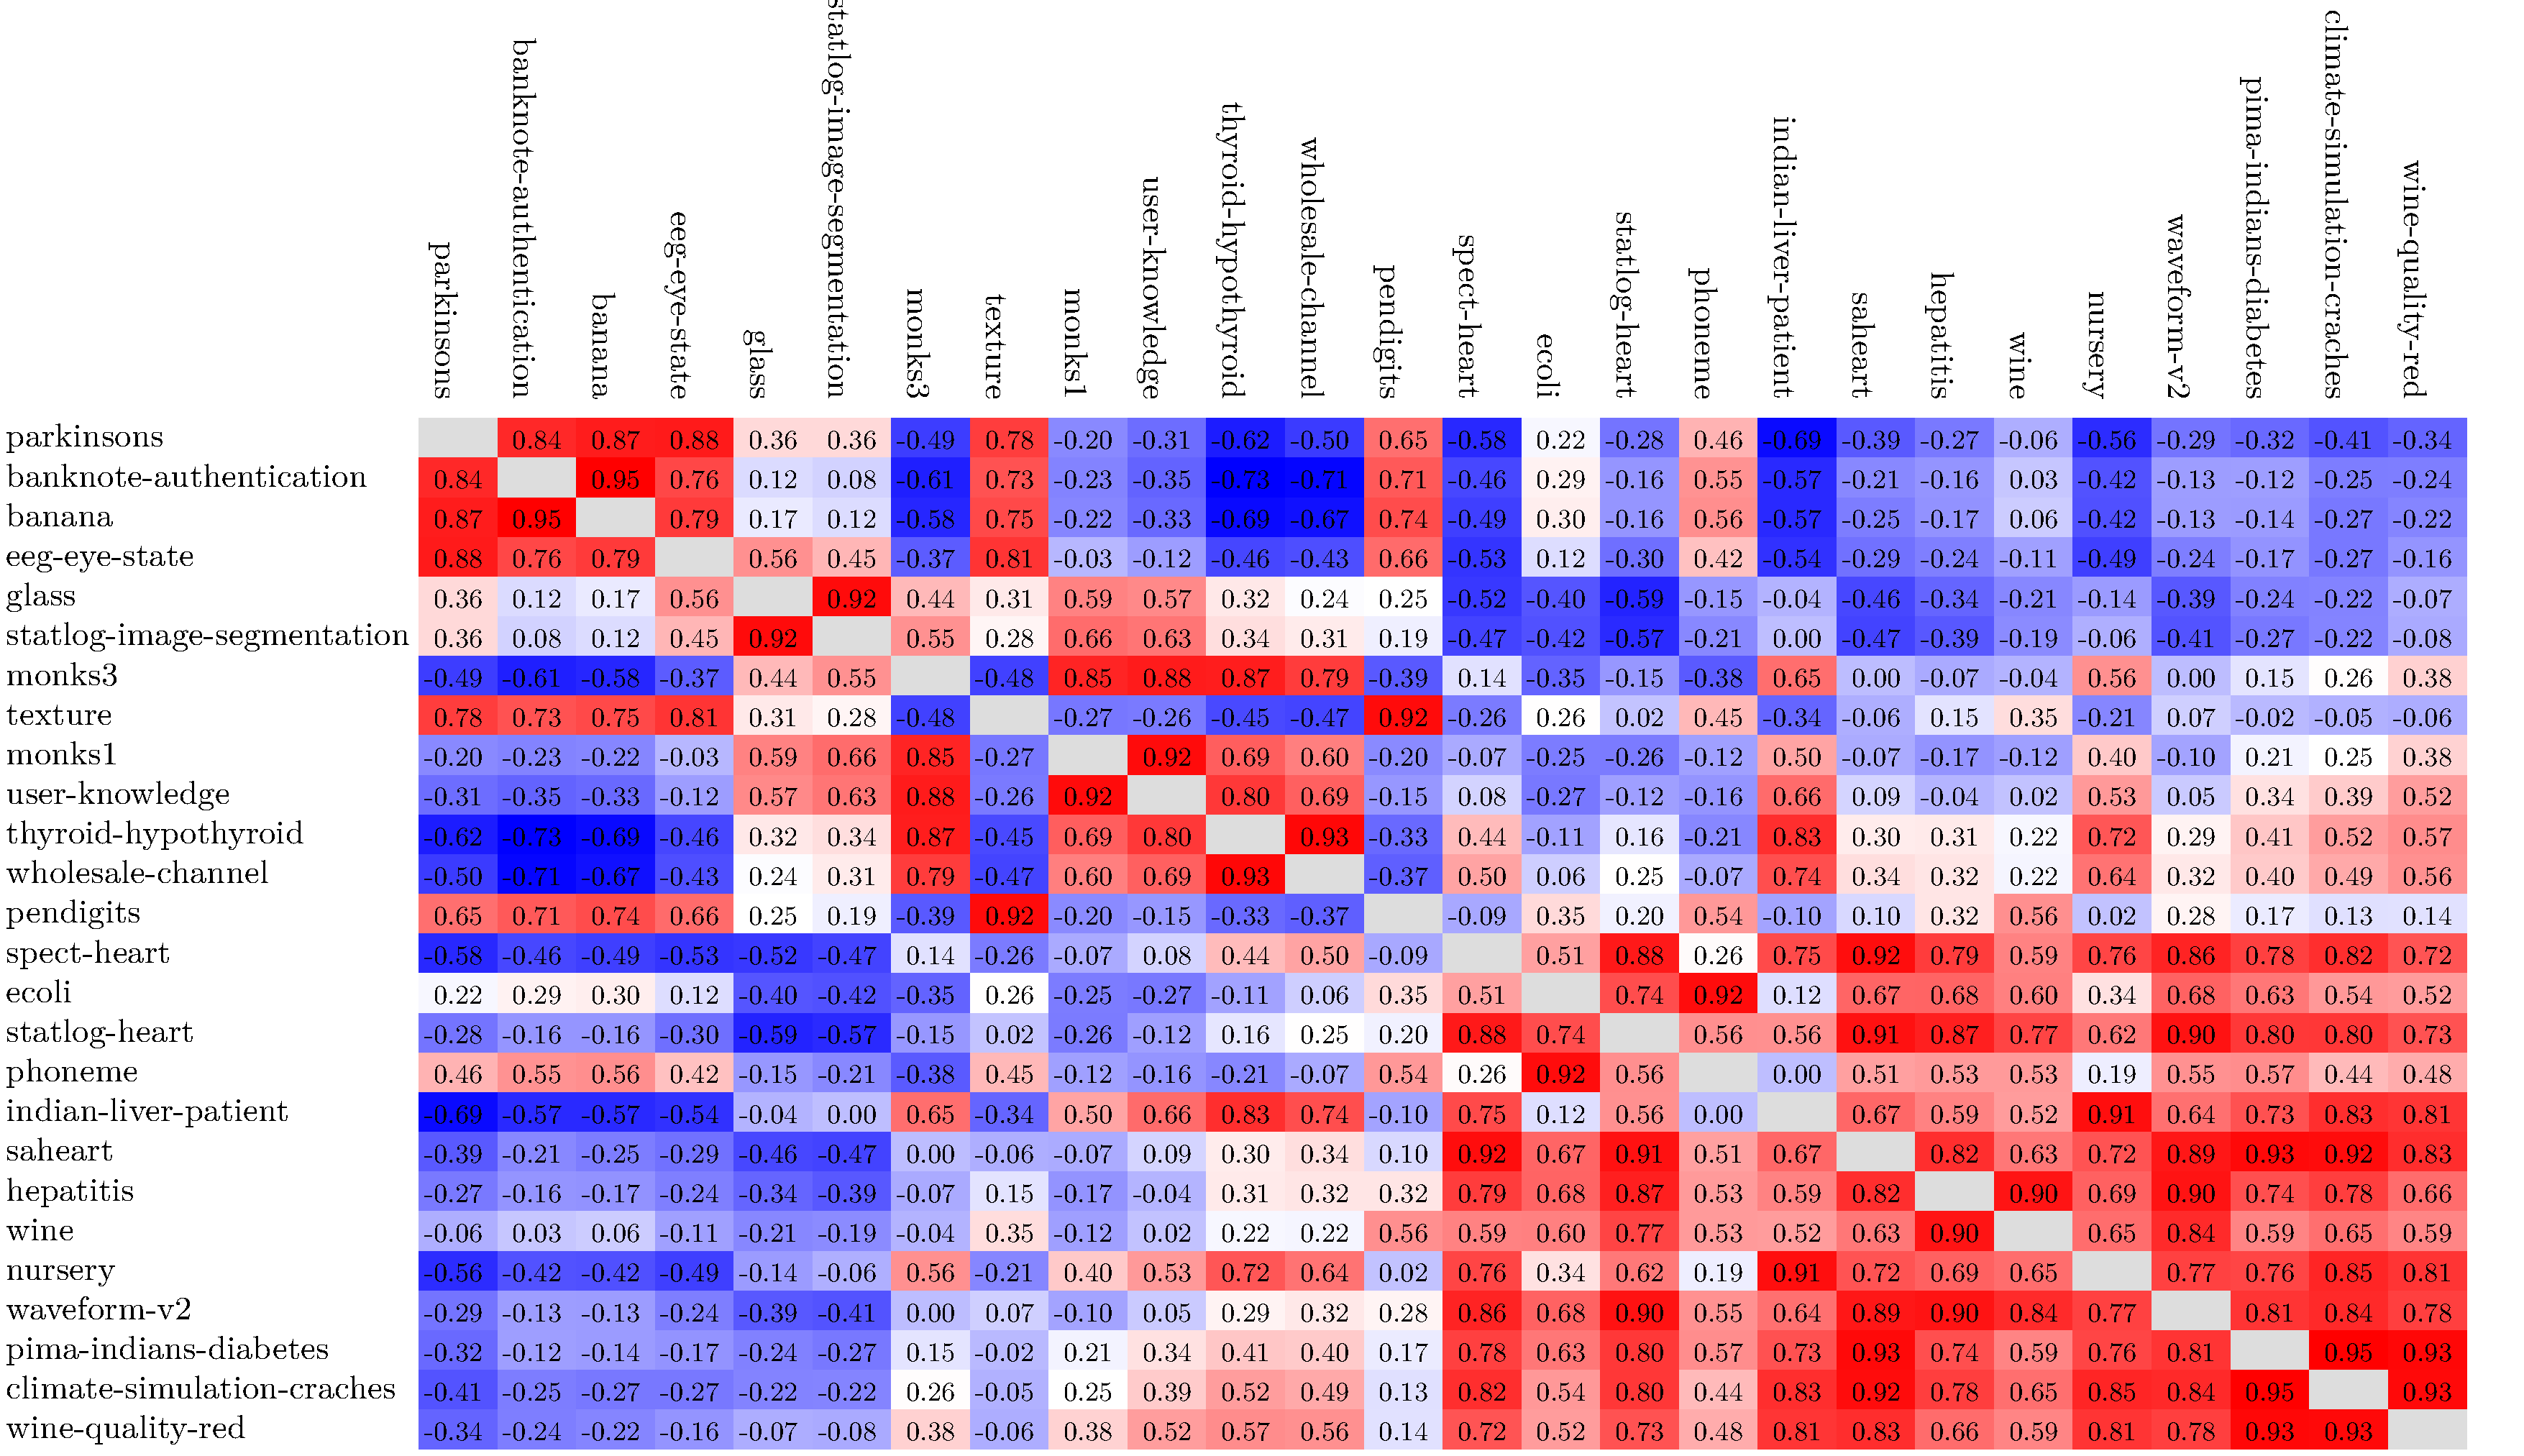
\includegraphics[scale=0.43]{images/heatmap-final-datasets.pdf}
  \caption[Valores de correlação entre conjuntos de dados mais correlacionados.]{
Valores de correlação entre os conjuntos de dados mais correlacionados.
}
  \label{datasetsimis}
\end{figure}
\end{landscape}
Variações como \textit{thyroid-sick-euthyroid} e \textit{thyroid-hypothyroid} ou \textit{volcanoes-d1} e \textit{volcanoes-e1} foram consideradas do mesmo domínio, porém como problemas distintos.
Na Tabela \ref{heatpares}, é possível observar que os domínios começam a coincidir somente com correlações abaixo de 0,830, havendo 18 pares de domínios distintos acima desse valor.
Logo, foi suposto que abaixo desse valor a coincidência de domínios fosse pouco preocupante.
Entretanto, análises posteriores ao término da presente pesquisa (Apêndice \ref{apflu}) indicam que seria fundamental manter apenas um conjunto de dados por domínio, para que a generalidade do aprendiz meta-ativo pudesse ser verificada.
\begin{table}
\caption[Pares de conjuntos com as maiores correlações.]{Pares de conjuntos com as maiores correlações. \textit{Pares em negrito relacionam conjuntos de domínios possivelmente próximos. Linha pontilhada simples indica omissão de pares de conjuntos de domínios distintos. Linha pontilhada dupla indica omissão de pares em geral.}}
\label{heatpares}
\centering\scalebox{0.842}{
\begin{tabular}{llr}
 \toprule
 \textbf{Primeiro conjunto} & \textbf{Segundo conjunto} &  \textbf{Correlação} \\
 \midrule
banana                             & banknote-authentication            & 0,950\\
climate-simulation-craches         & pima-indians-diabetes              & 0,949\\
pima-indians-diabetes              & wine-quality-red                   & 0,944\\
thyroid-hypothyroid                & wholesale-channel                  & 0,941\\
climate-simulation-craches         & wine-quality-red                   & 0,940\\
monks1                             & user-knowledge                     & 0,932\\
pima-indians-diabetes              & saheart                            & 0,926\\
saheart                            & waveform-v2                        & 0,924\\
pendigits                          & texture                            & 0,921\\
saheart                            & statlog-heart                      & 0,912\\
ecoli                              & phoneme                            & 0,912\\
glass                              & statlog-image-segmentation         & 0,909\\
indian-liver-patient               & nursery                            & 0,906\\
saheart                            & spect-heart                        & 0,903\\
eeg-eye-state                      & parkinsons                         & 0,903\\
hepatitis                          & wine                               & 0,902\\
monks3                             & user-knowledge                     & 0,900\\
statlog-heart                      & waveform-v2                        & 0,900\\
\textbf{thyroid-ann                        } & \textbf{thyroid-hypothyroid                }& 0,829\\ \hdashline
\textbf{vertebra-column-2c                 } & \textbf{vertebra-column-3c                 }& 0,821\\ \hdashline
\textbf{statlog-german-credit              } & \textbf{statlog-heart                      }& 0,821\\ \hdashline
\textbf{statlog-image-segmentation         } & \textbf{statlog-vehicle-silhouettes        }& 0,776\\ \hdashline
\textbf{autoUniv-au6-cd1               } & \textbf{autoUniv-au7-700                   }& 0,744\\ \hdashline
\textbf{thyroid-hypothyroid                } & \textbf{thyroid-sick-euthyroid             }& 0,740\\ \hdashline
\textbf{wine-quality-red                   } & \textbf{wine-quality-white-5class          }& 0,712\\ \hdashline
\textbf{volcanoes-d1                       } & \textbf{volcanoes-e1                       }& 0,712\\ \hdashline
\textbf{robot-failure-lp5                  } & \textbf{robot-nav-sensor-readings-2        }& 0,618\\ \hdashline
\textbf{volcanoes-b5                       } & \textbf{volcanoes-d1                       }& 0,606\\ \hdashline
\textbf{wine                               } & \textbf{wine-quality-red                   }& 0,590\\ \hdashline
\textbf{connectionist-mines-vs-rocks       } & \textbf{connectionist-vowel                }& 0,503\\ \hdashline
\textbf{volcanoes-b5                       } & \textbf{volcanoes-e1                       }& 0,500\\ \hdashline 
\hdashline
\textbf{autoUniv-au6-cd1-400               } & \textbf{autoUniv-au7-300-drift-au7,,,}& 0,000\\ \hdashline
\hdashline
\textbf{statlog-heart                      } & \textbf{statlog-image-segmentation         }& -0,524\\ \hdashline
robot-nav-sensor-readings-2        & seeds                              & -0,888\\
\bottomrule
\end{tabular}}
\end{table}

\subsection{Descrição}\label{descdatasets}
Todos os conjuntos selecionados, após particionamento dos dados durante o processo de validação cruzada, oferecem uma reserva com pelo menos 100 exemplos.
% $|\mathcal{U}|\geq 100$
Essa quantidade corresponde a um padrão de quantidade de consultas permitidas, de modo que as curvas de aprendizado de todos os conjuntos de dados sejam comparáveis entre si.
Os conjuntos têm suas características expostas no Apêndice \ref{apdatasets} - tabelas \ref{tab:datasetsa} e \ref{tab:datasetsb}.
Para ilustrar a diversidade dos conjuntos, alguns grupos especiais foram criados da seguinte forma:
\begin{itemize}
 \item classe majoritária 20 vezes mais numerosa que a classe minoritária (Tabela \ref{tab:imb});
 \item 60 ou mais atributos (Tabela \ref{tab:x});
 \item mais de 6 classes (Tabela \ref{tab:y});
 \item mais de 4000 exemplos (Tabela \ref{tab:n}); e,
 \item menos de 200 exemplos (Tabela \ref{tab:nm}). 
\end{itemize}

\input tex/dataset-tables-reduxes

Devido à presença de atributos nominais e numéricos, os algoritmos providos pela ferramenta Weka \cite{journals/sigkdd/HallFHPRW09} fizeram eventual uso de seus próprios filtros internos para lidar com cada tipo de atributo de acordo com a natureza do algoritmo: binarização, discretização e \ing{padronização}{z-score} \cite{kreyszig2007advanced}.
% Os algoritmos SVM e RoF (Seção \ref{learners}) requereram aplicação dos filtros externamente devido a incompatibilidade de seus filtros internos com alguns conjuntos de dados.

Exemplos duplicados foram removidos visando simular um oráculo consistente.
A cada grupo de exemplos repetidos, um único representante foi mantido cuja classe atribuída foi a moda das classes contempladas pelo grupo.

\section{Algoritmos de aprendizado}\label{learners}
Cada algoritmo de aprendizado tem, intrinsecamente, um viés próprio (Apêndice \ref{apmeta}) que, quando integrado a uma estratégia de amostragem ativa, pode influenciar no desempenho da estratégia.
Dessa forma, diferentes algoritmos foram adotados na comparação de estratégias.

As implementações adotadas são aquelas presentes na biblioteca Weka:
\sigla{\textit{k}-NN}{\textit{k}-vizinhos mais próximos}\footnote{Chamado IBk na implementação Weka.};
\sigla{C4.5w}{árvore de decisão C4.5}\footnote{Chamado J48 na implementação Weka.};
NB (\textit{Naive Bayes}); e,
\textit{Support Vector Machines} (SVM)\footnote{Invólucro LibSVM para Weka.}
\cite{journals/tit/Hart68,
books/mk/Quinlan93,
conf/ecml/Lewis98,
hearst1998support}.
O sufixo \textit{w} foi acrescentado como indicativo de que a implementação Weka não corresponde diretamente ao algoritmo original.

Algoritmos que requeiram ajuste externo de parâmetros frequentemente dependem de métodos de seleção de modelo \cite{arlot2010survey}.
Entretanto, no cenário de aprendizado ativo, o conjunto de treinamento é pequeno durante a maior parte da curva de aprendizado, tornando a seleção de modelos pouco confiável.
Adicionalmente, a complexidade dos métodos de seleção de modelo é computacionalmente incompatível com a necessidade de induzir um novo modelo a cada nova consulta.
Por fim, tendo em vista que o objetivo da seleção de algoritmos descrita nesta seção não foi a maximização da acurácia de algum algoritmo em particular, mas fornecer uma diversidade de vieses de aprendizado, não era mandatório que os parâmetros fossem otimamente ajustados.
Consequentemente, optou-se por valores pré-definidos.
O ajuste de parâmetros foi feito de acordo os valores padrão das implementações e as necessidades do aprendizado ativo, conforme listado a seguir.
\begin{itemize}
   \item \textit{k}-NN (denominado 5NN daqui em diante) - A quantidade adotada de 5 vizinhos possibilitou uma estimação de probabilidades com uma resolução que permite 6 valores quando todos os exemplos estão à mesma distância: 
   \[P_{\theta}(y|\bm{x}) \in \{0,0; 0,2; 0,4; 0,6; 0,8; 1,0\} \forall \bm{x} \in X, y \in Y\]
   Quanto maior a resolução, mais detalhada é a comparação de medidas de informatividade.
O voto de cada vizinho foi ponderado por $1 - d$ para atenuar as estimativas de probabilidade, onde $d$ é a distância euclidiana padronizada \cite{kreyszig2007advanced}.
\item C4.5w - A ramificação dos nós de decisão foi múltipla (não apenas binária), com fator de confiança na poda $0,25$ e % (smaller values incur more pruning)
um valor mínimo de 2 exemplos por folha.
A poda se deu com a \ing{substituição de nós por folhas}{subtree replacement}.
A estimação de probabilidades foi realizada com suavização aditiva \cite{books/daglib/0021593}, com o objetivo de atenuar as medidas de informatividade.
	\item NB - Uma discretização supervisionada de atributos numéricos foi realizada antes de cada treinamento \cite{conf/ijcai/FayyadI93}.
	\item SVM - Tipo C-SVC \cite{journals/ml/CortesV95} com núcleo função de base radial.
Os parâmetros, de acordo com a notação usual na literatura de SVM, seguiram os seguintes valores: $\gamma=0,5$;
% \item cache 200MB
% Shrinking(false)
% ProbabilityEstimates(true)
$C=1$; e, $\epsilon=0,001$ (tolerância do critério de parada). %SVMmulti eps=0,1

%inverse of the radius of influence of support vectors
% classif/learner g=0.5; SVMmulti g=1
%A low C makes the decision surface smooth, high C aims at classifying all training examples correctly
\end{itemize}

Um experimento envolvendo comitês também foi realizado.
Eles são apresentados na Seção \ref{algensembles}.

\subsection{Comitês}\label{algensembles}
Um comitê de classificadores é composto por diversos modelos visando um aumento na acurácia preditiva (Seção \ref{qbc}).
Um efeito colateral está na geração de estimativas de probabilidade mais tênues por serem baseadas na sumarização de predições feitas por modelos distintos e, em algum grau, independentes.
Estratégias de amostragem ativa baseadas na incerteza do modelo podem se beneficiar de predições atenuadas, pois elas podem aumentar seu poder discriminatório durante a comparação de exemplos para consulta.
Esse benefício é mais notável quando o algoritmo tende a gerar modelos excessivamente confiantes.
Segundo \citeonline{conf/icml/RoyM01}, o algoritmo NB, por exemplo, produz estimativas de probabilidade erroneamente elevadas para exemplos de fronteira quando sua premissa de independência entre os atributos é quebrada.
Uma solução proposta por esses autores é a adoção de um comitê do tipo \textit{bagging} (Seção \ref{qbc}).

Visando aumentar a abrangência dos resultados, optou-se, aqui, pela inclusão de um experimento com comitês.
Dois comitês equiparáveis e com desempenho geral elevado \cite{journals/jmlr/DelgadoCBA14} foram escolhidos: \sigla{RoF}{\textit{Rotation Forest}} e \sigla{RFw}{\textit{Random Forest}}
% Delgado: 121 datasets
\cite{journals/pami/RodriguezKA06,journals/ml/Breiman01}.
% RFw não realiza poda e faz a escolha aleatória de $\log_2|A| + 1$ atributos por árvore.
A escolha desses dois algoritmos permitiu a realização de um experimento com a acurácia preditiva num patamar superior à que foi obtida no experimento de modelos únicos.
Os comitês foram configurados com apenas 10 membros, devido às limitações de recursos computacionais anteriormente mencionadas (Seção \ref{sectempo}).

Nesta tese, comitês também foram aplicados a uma tarefa de regressão, que consistiu na predição de ranqueamentos pelo algoritmo \sigla{PCT}{\textit{Predictive Clustering Trees}} para o sistema de recomendação automática - introduzido na Seção \ref{algmeta}.

\subsection{Diversidade de algoritmos}
O mesmo procedimento experimental da Seção \ref{secsimi} foi adotado para avaliar a similaridade entre os algoritmos de aprendizado,
com exceção da medida de correlação, que foi substituída pela distância de Hamming \cite{hamming1950error}.
Essa métrica quantifica as predições distintas entre cada par de modelos para uma dada coleção de conjuntos de dados.
Ela representa diretamente o grau de equivalência entre algoritmos do ponto de vista da predição de classes.
Logo, é mais precisa que a medida anterior (Seção \ref{secsimi}).

O algoritmo 5NN foi testado com duas métricas de distância e com a opção de ponderação.
A versão com ponderação (indicada nesta seção pelo sufixo \textit{p}) foi preferida por permitir estimativas de probabilidade atenuadas, necessárias para parte das estratégias de amostragem ativa.
As versões com a distância de Manhattan (indicada pelo sufixo \textit{m}) foram descartadas devido à excessiva semelhança com as versões baseadas na distância euclidiana, pois obteve valores 0 e 13 no cálculo da distância de Hamming - conforme Figura \ref{leasimis}.
\begin{figure}
  \setlength{\unitlength}{1.0cm}
  \centering
    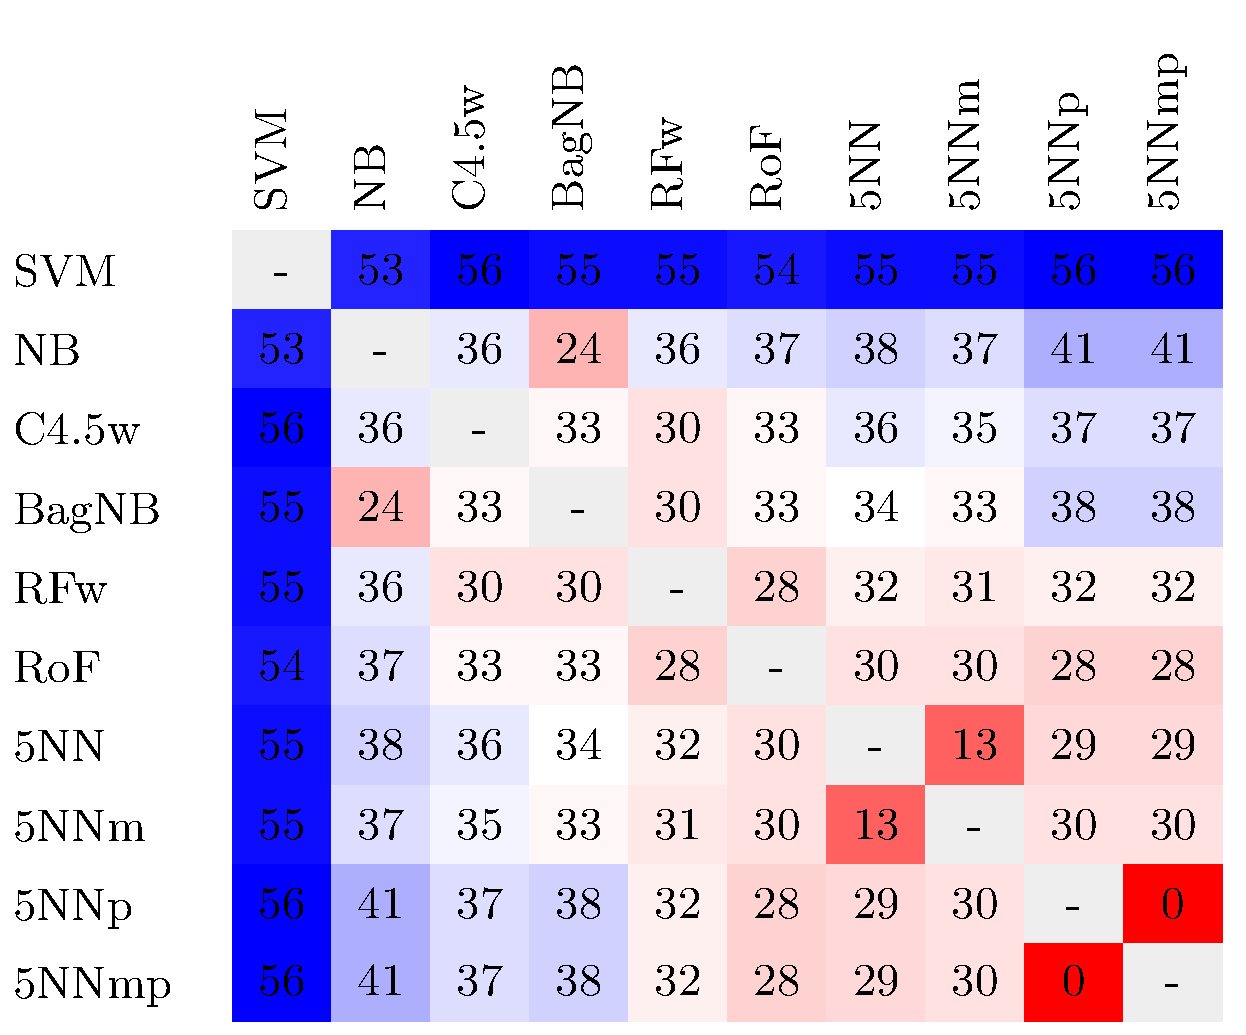
\includegraphics[scale=0.45]{images/heatmap-final-leas.pdf}
  \caption[Média da distância de Hamming entre predições de modelos induzidos]{Média da distância de Hamming entre as predições de modelos induzidos por diferentes algoritmos.}
  \label{leasimis}
\end{figure}



\subsection{Algoritmos de (meta) aprendizado}\label{algmeta}

É esperado que apenas parte dos 53 meta-atributos definidos na Seção \ref{sec:ama} seja relevante na tarefa de predição de ranqueamento ou recomendação de algoritmos.
Logo, os algoritmos de aprendizado mais apropriados são aqueles capazes de lidar com atributos irrelevantes.
Um tipo de algoritmo com essa capacidade frequentemente empregado é o comitê de árvores \cite{strobl2009introduction}.
Quatro algoritmos baseados em comitê de árvores com relatos de alto desempenho em geral \cite{journals/jmlr/DelgadoCBA14} frente a outros algoritmos são RFw, RoF (Seção \ref{algensembles}), \textit{Predictive Clustering Trees} (PCT) e, não necessariamente baseado em árvores, \sigla{ABoo}{AdaBoost} - \cite{journals/jmlr/DelgadoCBA14,conf/icml/FreundS96,conf/ecml/TodorovskiBD02}.
Eles foram adotados para gerar os modelos de recomendação do sistema de meta-aprendizado.
O prefixo \textit{meta} é acrescentado para desfazer qualquer ambiguidade entre o nível base e o nível meta - exemplos de uso: \ul{meta}PCT, EERent-\ul{meta}RoF, \ul{meta}-aprendiz, \ul{meta}classe, \ul{meta}exemplos, \ul{meta}conjunto de dados etc.

Optou-se pela quantidade padrão de 500 membros definido na implementação do algoritmo \textit{Random Forest} para a linguagem R \cite{team2014r}.
Esse número foi considerado válido pelos seguintes motivos:
\begin{itemize}
   \item é importante garantir que a quantidade de membros seja grande o bastante para não haver perda de acurácia devido a falta de membros - 128 árvores foram suficientes para atingir a acurácia máxima numa coleção de 29 conjuntos de dados, segundo \citeonline{conf/mldm/OshiroPB12};
%http://download.springer.com/static/pdf/998/chp%253A10.1007%252F978-3-642-31537-4_13.pdf?originUrl=http%3A%2F%2Flink.springer.com%2Fchapter%2F10.1007%2F978-3-642-31537-4_13&token2=exp=1446670434~acl=%2Fstatic%2Fpdf%2F998%2Fchp%25253A10.1007%25252F978-3-642-31537-4_13.pdf%3ForiginUrl%3Dhttp%253A%252F%252Flink.springer.com%252Fchapter%252F10.1007%252F978-3-642-31537-4_13*~hmac=d7f4c13c3879943df0e5b9f9f9fc8da7066cef8851e5fd261f98bee18f8a35c7
% as the number of trees grows, it does not always mean the performance of the forest is significantly better than previous forests (fewer trees), and doubling the number of trees is worthless. It is also possible to state there is a threshold beyond which there is no significant gain, unless a huge computational environment is available.
   \item o fator determinante na escolha do tamanho do comitê é o custo computacional \cite{conf/mldm/OshiroPB12};
   \item o risco de sobreajuste nesse parâmetro é baixo ou inexistente devido ao \textit{paradoxo da generalização do comitê} \cite{elder2003generalization,series/synthesis/2010Seni};
   \item é uma quantidade computacionalmente viável para o experimento do nível meta; e,
   \item sendo um número padrão, facilita a replicabilidade ou comparação com resultados de terceiros.
\end{itemize}

% A heurística de PCT para a definição de regras nos nós é a redução da variância.
%       "FTest = 1") ++
%       (if (ntrees == 1) Seq("PruningMethod = M5Multi", //ajuda C45 quebra
%         "M5PruningMult = 1", "")
%       else Seq("")) ++ //ajuda mais
        
\section{Estratégias}\label{confstrats}

Nos experimentos realizados, 9 estratégias e 5 variantes foram avaliadas.
O conjunto de estratégias selecionadas foi considerado representativo da diversidade de paradigmas relevantes de aprendizado ativo, de acordo com os artigos referenciados por \citeonline{series/synthesis/2012Settles}.

Foram acrescentados os sufixos \textit{euc} e \textit{man} nas siglas de estratégias que façam uso das distâncias euclidiana e de Manhattan, respectivamente.
Os sufixos \textit{ent} e \textit{acu} indicam, respectivamente, os critérios de entropia e de acurácia balanceada para a estratégia EER (baseada na \textit{redução do erro esperado}).
Dentre as possibilidades iniciais, três estratégias foram descartadas.
SVMsim e SVMbal foram implementadas (Seção \ref{outras}), mas descartadas dada a sua dependência de um algoritmo específico e seu desempenho excessivamente baixo em testes iniciais - possivelmente devido a um insucesso da adaptação multiclasse escolhida.
QBC (\textit{Query By Committee}) foi implementada para o comitê RFw com a medida $\JS$ (Seção \ref{outras}), mas também descartada pelos mesmos motivos.
% journals/jmlr/BaramEL04 foram adaptados para contemplar problemas multiclasse por meio da aplicação de \ing{rodízio}{round-robin} entre sub-estratégias. A cada sub-estratégia foi atribuída uma classe principal na configuração \textit{um para muitos}.

Um conjunto reduzido de estratégias foi utilizado na parte inicial da análise comparativa (Seção \ref{despred}).
Assim, somente uma variante por estratégia foi selecionada para esse primeiro momento.
As variantes não incluídas foram as seguintes:
\begin{itemize}
%    \item DW (DWeuc e DWman) \ano{sigla} - DW é conceitualmente e experimentalmente inferior a TU \cite{bracis15}, cujo paradigma \ano{termo} a representa parcialmente;
   \item ATUman, DWman, TUman e HTUman (todas as estratégias baseadas em densidade) - a distância euclidiana foi considerada mais usual que a distância de Manhattan, cujo desempenho, em geral, é similar \cite{bracis15}; e,
   \item EERacu - a variante EERent foi preferida porque $E$ (entropia) é a medida proposta no trabalho original.
\end{itemize}

Algumas das estratégias exigiram configurações específicas.
As escolhas adotadas nessas configurações são detalhadas nas seções seguintes.

\subsection{EERent e EERacu} \label{eerconfig}
A utilização da acurácia balanceada \cite{journals/bmcbi/MassoV10} como função objetivo alternativa configurou-se como uma variação do método (EERacu), visando agir diretamente na medida de interesse nos experimentos (Seção \ref{medidas}).
A acurácia balanceada foi preferida à $\kappa$ por ser uma medida multiclasse com menos propensão a ter valores próximos ou iguais a zero, evitando, assim, o anulamento da medida de informatividade.
Apenas 100 exemplos foram aleatoriamente amostrados de $\mathcal{U}$ antes de cada consulta para reduzir o alto custo computacional de EER.

\subsection{HS}\label{metohs}
A implementação original do autor foi empregada neste trabalho com o mesmo
algoritmo de agrupamento, 
\textit{Ward's average linkage method}\footnote{
Implementação disponível no Weka \cite{journals/sigkdd/HallFHPRW09}.}.

\subsection{DW, TU, ATU e HTU}
Os parâmetros de ponderação foram fixados no valor 1 ($\alpha=1$, $\delta=1$).

\section{Avaliação}\label{avaliacao}
A avaliação dos resultados experimentais foi realizada qualitativamente por meio de curvas de aprendizado e quantitativamente por meio de medidas de desempenho (Seção \ref{medidas}).
As formas de validação são apresentadas na Seção \ref{validacao}.
A parte quantitativa foi confirmada por testes estatísticos (seções \ref{testestbase} e \ref{testestmeta}). 

\subsection{Medidas}\label{medidas}
Nos experimentos desta tese, foram necessárias medidas de avaliação de desempenho preditivo específicas para o nível base e para o nível meta.
Essas medidas são apresentadas nas seções seguintes.

\subsubsection{Nível base}\label{metrbase}
\simbolo{\mu_\kappa}{valor médio de $\kappa$ para 5 execuções de validação cruzada em 5 partes}
\simbolo{\sigma_\kappa}{desvio padrão de $\kappa$ para 5 execuções de validação cruzada em 5 partes}
% Settles (com f-measure e sem log(x))
% An analysis of active learning strategies for sequence labeling tasks (2008)
% No "active chalenge 2011", que alguns adotam como referência para citar ALC, foi usada a AUC verdadeira e log2(x) no cálculo (igual ao Cawley):
% http://www.causality.inf.ethz.ch/activelearning.php?page=evaluation
% Porém, eles avaliam sem validação cruzada, talvez por limitação do próprio fato de ser uma competição.
% O dataset inteiro é usado uma só vez e o teste é feito em cima de
% "all the samples with unknown labels".
% Isso explica o fato de classificadores semisupervisionados terem alavancado as estratégias na competição.

Uma medida de desempenho preditivo comumente utilizada na área de aprendizado ativo é a \ing{\sigla{ALC}{área debaixo da curva de aprendizado}}{Area under the Learning Curve}.
Uma das primeiras menções a esse tipo de medida em aprendizado ativo, até onde o conhecimento do autor permite dizer, foi feita por \citeonline{raghavan2007will}.
A medida ALC foi empregada em diversos artigos, como no trabalho de \citeonline{conf/emnlp/SettlesC08} e aplicado em momentos relevantes, como na competição de aprendizado ativo mencionada no Capítulo \ref{intro}.

A ALC é o valor resultante do somatório de alguma medida de desempenho ao longo das consultas.
Seu intuito é avaliar o desempenho geral de uma estratégia, ou seja, em uma ampla faixa de orçamentos.
Logo, a medida se mostra adequada para os objetivos desta tese, relacionados à comparação de estratégias.
Neste trabalho, ela foi adotada em conjunto com a extensão do índice kappa de Cohen, $\kappa$ - detalhada na Seção \ref{newhtu}.
Na descrição dos resultados, os valores de ALC apresentados são o resultado da divisão da ALC pela quantidade de consultas, visando manter a interpretabilidade da medida.

O índice $\kappa$ é utilizado para comparar o grau de consenso entre avaliadores \cite{journals/coling/EugenioG04}.
Seu poder discriminatório tem sido satisfatório frente a outras medidas de sumarização da matriz de confusão \cite{conf/acivs/DemirkesenC08}.
Quando aplicado como medida de desempenho de classificação, o valor limite $1$ indica acerto total, $0$ desempenho equivalente ao aleatório e $-1$ erro total. Entretanto, nem sempre o limite inferior coincide com $-1$ \cite{journals/ese/Emam99}.
Esse índice permite realizar a comparação sob dois pontos de vista: entre estratégias (valor relativo) e em relação ao acaso (valor absoluto).

Dada a presença de um alto grau de desbalanceamento entre as classes nos conjuntos de dados da coleção, a medida de acurácia convencional seria uma medida de desempenho inadequada, pois permitiria que a classe majoritária dominasse a composição de seu valor final.
De fato, as proporções das classes majoritária e minoritária chegam a extremos de, respectivamente, $96,5\%$ e $0,0\%$ (1 exemplo) do tamanho da reserva - conforme Tabela \ref{tab:imb}.

As curvas de aprendizado e valores de ALC são baseadas nas médias das curvas resultantes de um procedimento de validação cruzada \cite{settles2010active}.
Cada curva exibe a medida de interesse $\kappa$ em função da quantidade de consultas.
Assim, neste texto,  o valor médio $\mu_{\kappa}$ de $\kappa$ para as 5 execuções de validação cruzada em 5 partes (Seção \ref{validacao}) é a medida base de todos os resultados sobre desempenho relacionado à capacidade preditiva.
%neste documento.
Como consequência, cada conjunto de dados tem um valor de $\mu_{\kappa}$ e seu correspondente desvio padrão $\sigma_{\kappa}$ para cada consulta de uma dada estratégia.
É importante diferenciar $\mu_{\kappa}$ (e $\sigma_{\kappa}$), que é uma média de valores $\kappa$ interna a cada conjunto de dados, da \textit{média de} $\mu_{\kappa}$ (e \textit{média de} $\sigma_{\kappa}$), que é calculada para a coleção como um todo.
% Logo, referências à \textit{média de} $\bar{\kappa}$ e ao \textit{desvio padrão de} $\bar{\kappa}$ indicam as estatísticas sobre $\bar{\kappa}$ em relação a todos os 90 conjuntos de dados.

\subsubsection{Nível meta}\label{avmeta}
A avaliação do sistema de recomendação foi realizada conforme dois cenários:
classificação 
% (metaestratégia/recomendação do melhor algoritmo)
e predição de ranqueamento de algoritmos.
% (estimação da colocação de cada candidato).
Seguindo a escolha de \citeonline{conf/ijcnn/SoutoPSACLS08}, a predição pelo \sigla{Def}{ranqueamento médio} foi uma das referências utilizadas na avaliação do sistema de recomendação.
O \sigla{Alea}{ranqueamento aleatório} e a \sigla{Maj}{escolha fixada na classe majoritária} também serviram de referência.
A comparação entre as predições de ranqueamento foi feita por meio do cálculo do coeficiente de correlação de Spearman (Seção \ref{secsimi}).
O desempenho de classificação foi avaliado pela comparação da medida $\kappa$ e, paralelamente, pelas acurácias ordinária e balanceada na predição de melhor algoritmo de aprendizado.
A mesma metodologia foi adotada na investigação inicial de outras possibilidades de recomendação: de estratégias de amostragem ativa, de pares estratégia-algoritmo, de métricas de distância para estratégias baseadas em densidade e da própria utilização ou não de aprendizado ativo.

Para verificação da efetividade do sistema de recomendação, o efeito do meta-aprendiz também foi avaliado no nível base.
O algoritmo para o papel de aprendiz para cada dada estratégia foi escolhido automaticamente e seu desempenho foi comparado diretamente com os demais algoritmos no nível base por meio dos valores de ALC e curvas de aprendizado.

\subsection{Validação}\label{validacao}
Não há consenso na literatura de aprendizado ativo sobre a melhor maneira de validação.
% Uma consulta por ``cross-validation'' e ``active learning'' no google scholar em 12/10/15 retornou parte dos seguintes resultados mais referenciados diretamente relacionados à presente pesquisa.
Dados os recursos disponíveis, optou-se por 5 execuções de validação cruzada em 5 partes.
Ela tem uma menor variabilidade quando comparada à \sigla{LOO}{\textit{Leave-One-Out}} e à validação em 10 partes \cite{journals/neco/KearnsR99} e um menor enviesamento quando comparada, por exemplo, com a validação em 2 partes ou \textit{hold-out} \cite{arlot2010survey}.
Adicionalmente, a validação em 5 partes é uma configuração comum na literatura.
Algumas das possibilidades encontradas em trabalhos relevantes são as seguintes:
\begin{itemize}
 \item validação em conjunto à parte pré-definido pelos autores dos conjuntos de dados \cite{conf/cikm/ErtekinHBG07};
 \item 100 execuções de validação em conjunto com 40\% dos exemplos à parte \cite{journals/jmlr/BaramEL04}; % For almost all problems, this collection includes 100 folds each consisting of a fixed 60\%/40\% training/test partition.
 \item validação cruzada em 5 partes \cite{chen2015study,settles2008active,conf/ecml/LomaskyBAWF07,conf/ecir/XuAZ07}; % we used a 5-fold CV to assess accuracy. % we pursue 5-fold cross-validation on the Active-RDD algorithm and Gapped Top K algorithm, and compare their cross-validation performance (CVP) with Cluster Centroid and Top K algorithm performance,(these algorithms are consequently parameter free in this setting). We separate 50 queries into 5 parts, where each part contains 10 queries. For the kth set of queries, we train parameters to optimize the retrieval performance for the other 4 sets of queries, and use this set of the parameters to test on kth set of queries to obtain the retrieval performance measure for kth part. We do this for k = 1, 2, 3, 4, 5 and the cross-validation performance is the average performance on the 5 test query sets. The cross-validation experimental results are shown in Table 2.   
 \item 4 execuções de validação cruzada em 5 partes \cite{conf/ijcai/BeckerO05,conf/icml/MusleaMK02}; % We report the average over a 5-fold cross-validation to ensure statistical significance of the results. In a single fold, we randomly sample (without replacement) an initial labelled training set of a fixed size – 500 or 2,000 sentences, depending on the experiment – and a test set of 1,000 sentences. The remaining sentences constitute the global pool of unlabelled sentences (ca. 37,000 sentences) % four runs of 5-fold cross-validation.
 \item validação cruzada em 9 partes \cite{conf/iswc/StikicLS08}; % As suggested in [12], we use 9-fold leave-one-day-out cross validation on the data to avoid over-fitting. In each cross validation round of supervised learning, we train the algorithms on 8 days of data. In case of semi-supervised and active learning, only a subset of 2 days of data is used as an initial labeled training set. The algorithms are always tested on the left out day’s data.
 \item validação cruzada em 10 partes \cite{settles2008active}; % baselines: the cost-sensitive method using known annotation times, and random sampling. The task-models are evaluated with the F1 measure and averaged using ten-fold cross-validation (five-fold for CKB).
 \item 2 execuções de validação cruzada em 10 partes \cite{conf/ecml/KornerW06,conf/icml/MelvilleM04}; e,% We initiated the active learners with 50 randomly drawn training instances and evaluated the experiments based on 2x10-fold cross validation. During each iteration we added 1 query to the training set and proceeded until all available data was used or a maximum of 250 queries. 
 \item validação cruzada em 20 partes \cite{conf/ijcai/MusleaMK03}. % we use 20-fold cross-validation to compare the performance 
\end{itemize}

No nível meta, LOO foi utilizada na avaliação do desempenho na predição de ranqueamentos conforme sugerido por \citeonline{journals/ml/BrazdilSC03}.
Essa abordagem maximizou a utilidade dos dados disponíveis, que correspondem a apenas 90 metaexemplos, um para cada conjunto de dados.
Além disso, LOO fornece a estimativa menos enviesada da acurácia quando comparada às demais formas de validação cruzada \cite{conf/icml/Joachims00} e, nesse contexto, permite a aplicação de teste estatístico, conforme discutido na Seção \ref{testestmeta}.

Por outro lado, no caso da avaliação do desempenho de classificação no nível meta, o teste estatístico não pôde ser aplicado com confiabilidade pelos motivos descritos na Seção \ref{testestmeta}.
Optou-se, então, por dez execuções de validação cruzada em dez partes \cite{conf/pakdd/BouckaertF04}, 

% A survey of cross-validation procedures for model selection (2010):
% http://www.di.ens.fr/willow/pdfs/2010_Arlot_Celisse_SS.pdf
% …
% As noticed in the early 30s by Larson (1931), training an algorithm and evaluating its statistical performance on the same data yields an overoptimistic result.
% CV was raised to fix this issue, starting from the remark that testing the output of the algorithm on new data would yield a good estimate of its performance(Mosteller and Tukey, 1968; Stone, 1974; Geisser, 1975).
% …
% Leave-one-out (LOO, Stone, 1974; Allen, 1974; Geisser, 1975) is the most classical exhaustive CV procedure.
% …
% LOO bootstrap and .632 bootstrap. … these procedures have nearly no theoretical justification and only empirical studies have supported the good behaviour of .632+ bootstrap
% 
% tem até review de fast CVs.
% ;;;
% PASSIVO: According to Breiman and Spector (1992) the best risk estimator is LOO,
% whereas 10-fold CV is more accurate for model selection.
% }

\subsection{Teste estatístico no nível base}\label{testestbase}
% from cerri: Para verificar a significância estatística dos resultados, foram empregados os testes de Friedman e Nemenyi, recomendados para comparações envolvendo vários métodos e muitos conjuntos de dados (Demšar, 2006). O teste de Friedman é um teste não paramétrico, pois não assume nada acerca da distribuição dos dados. Ele é baseado em rankings, e verifica se há diferença estatisticamente significante em um grupo de comparações. O teste de Nemenyi é um teste post-hoc aplicado após o teste de Friedman. Ele é utilizado para encontrar quais pares de comparações apresentam diferenças estatisticamente significantes. Nos testes estatísticos, foi utilizado um nível de confiança de 95%.
As diferenças de desempenho preditivo foram atestadas pelo teste não paramétrico de Friedman com teste post-hoc de Nemenyi seguindo a abordagem proposta por \citeonline{journals/jmlr/Demsar06} para comparações de classificadores.
Ainda conforme a abordagem do autor daquele estudo, os valores foram arredondados na terceira casa decimal, para forçar o empate nas diferenças irrelevantes.
Os resultados do teste são sumarizados numa tabela cujas células contêm símbolos que indicam com que nível de significância estatística uma estratégia na linha vence a outra na coluna.
No exemplo com algoritmos hipotéticos dado na Tabela \ref{exfried}, o algoritmo 1 vence o algoritmo 2 com $p\valor<0,01$; o algoritmo 2 vence o algoritmo 3 com $p\valor<0,05$ e o algoritmo 3 vence o algoritmo 4 com $p\valor<0,10$.
A contagem de ocorrências de primeiros e últimos lugares é apresentada na Tabela \ref{exconta}.
\begin{table}
\parbox[t][]{.48\linewidth}{\vspace{0pt}
	\flushright
	\caption[Exemplo com legenda das diferenças estatisticamente significativas.]{Exemplo de tabela de sumarização de diferenças estatisticamente significativas.
	\textit{Cada símbolo representa um nível de significância estatística $\alpha$:}
	* ($\alpha=0,01$), + ($\alpha=0,05$) e . ($\alpha=0,10$).}
	\label{exfried}
	\scalebox{0.9}{
	\begin{tabular}{lccccc}
	\toprule
						& 1 & 2 & 3 & 4 & 5 \\[4pt] \midrule
		1 - algoritmo 1	& - & * &   &   &   \\[4pt]
		2 - algoritmo 2	&   & - & + &   &   \\[4pt]
		3 - algoritmo 3 & 	&   & - & . &   \\[4pt]
		4 - algoritmo 4	&   &   &   & - &   \\[4pt]
		5 - algoritmo 5 & 	&   &   &   & - \\\bottomrule
	\end{tabular}
	}
}
\hfill
\parbox[t][]{.48\linewidth}{\vspace{0pt}
	\flushright
	\caption[Exemplo de contagem de colocações.]{Exemplo de contagem de colocações. Medida: ALC-$\sigma_{\kappa}$. \textit{O melhor e o pior valor de cada coluna estão em \textcolor{blue}{\textbf{negrito azul}} e \textcolor{red}{\textbf{negrito vermelho}} respectivamente. Apenas negrito indica segundo melhor valor.}}
	\label{exconta}
	\scalebox{0.9}{
	\begin{tabular}{lccc}
		\toprule
		 &\scriptsize \makecell{\textbf{Primeiras}\\\textbf{colocações}} &\scriptsize \makecell{\textbf{Últimas}\\\textbf{colocações}} \\
		\midrule              
		algoritmo 1& \bom{78} & \bom{13} \\
		algoritmo 2& \bomd{67} & \ruim{91} \\
		algoritmo 3& 55 & \bomd{24} \\
		algoritmo 4& 43 & 44 \\
		algoritmo 5& \ruim{35} & 44 \\
	\bottomrule
	\end{tabular}
	}
}
\end{table}
O critério de vitória é baseado na comparação dos valores de ALC de $\mu_{\kappa}$ (ALC-$\mu_{\kappa}$) para os dois algoritmos em questão em cada conjunto de dados.


\subsection{Teste estatístico no nível meta}\label{testestmeta}
% Dá quase pra deduzir da Nathalie que é possível aplicar Friedman em um só dataset sem quebrar (muito) as premissas.
% Mas isso não chega a ter o peso de uma prescrição. De qualquer forma, o conjunto é pequeno demais para isso (9 exemplos, se k=10).
As diferenças estatisticamente significativas entre metaPCT e Def foram reveladas pelo teste de Wilcoxon pareado \cite{journals/jmlr/Demsar06} aplicado aos valores de correlação entre os ranqueamentos esperados e seus correspondentes ranqueamentos preditos (Seção \ref{avmeta}).
Cada metaexemplo representa um conjunto de dados.
Logo, houve uma aproximação da premissa de \textit{independência entre amostras} devido ao isolamento de cada metaexemplo sob teste - situação intrínseca ao procedimento LOO.
Assim, a avaliação da predição de ranqueamento está estatisticamente fundamentada.

Por outro lado, a comparação de acurácias entre múltiplos metaclassificadores não permite aplicar um teste estatístico baseado em ranqueamento, quando há um único metaexemplo no conjunto de teste.
O motivo dessa impossibilidade é o valor da predição de classe ser discreto e, consequentemente, só poder ser avaliado como correto ou incorreto.
Outras coleções de conjuntos de dados precisariam ser incorporadas ao experimento,
mas isso não é viável com a presente disponibilidade de conjuntos pré-processados.
Entretanto, é possível obter valores informativos do metaconjunto que representa a única coleção disponível, caso seja alterada a forma de validação cruzada.
A média e o desvio padrão do desempenho preditivo podem ser obtidos por meio de dez execuções de validação cruzada em dez partes.

A troca da forma de validação é preferível, pois o desvio padrão retornado por LOO seria desprovido de significado prático.
Ele teria um valor elevado que refletiria o fato dele ser fruto do caso extremo em que o conjunto de teste tem apenas um elemento.
Além disso, quando há apenas um conjunto de dados e uma única execução, o desvio padrão obtido por LOO é mera função direta da acurácia.
Isso pode ser verificado no desenvolvimento das equações \ref{looeq} e \ref{looeq2}, onde $\mu$, $\sigma$, e $h_i \in \{0;1\}$ são, respectivamente, a acurácia média, seu desvio padrão e o valor correspondente a acerto (1) ou erro (0) para um dado exemplo de índice $i$.
A quantidade de acertos e o número de exemplos são dados por $a$ e $n$, respectivamente.
\begin{equation}\label{looeq}\mu = an^{-1} \end{equation}
\begin{equation}\label{looeq2}\begin{array} {lcl}
\sigma & = & \sqrt{\sum\limits_{1\leq i \leq n}(h_i - \mu)^2 n^{-1}} \\
&=&\sqrt{[a(1 - \mu)^2 + (n-a)(0 - \mu)^2] n^{-1}} \\
&=&\sqrt{[a - 2a\mu + \mu^2 + (n-a)\mu^2] n^{-1}} \\
&=&\sqrt{[a - 2a\mu + a\mu^2 + n\mu^2-a\mu^2] n^{-1}} \\
&=&\sqrt{[a - 2a\mu + n\mu^2] n^{-1}} \\
&=&\sqrt{an^{-1} - 2an^{-1}\mu + \mu^2} \\
&=&\sqrt{\mu - 2\mu^2 + \mu^2} \\
&=&\sqrt{\mu - \mu^2} \\
\end{array}\end{equation}
Adicionalmente, não seria possível contornar o problema por meio de múltiplas execuções, pois o procedimento LOO não dá margem para o acréscimo de perturbações na composição do conjunto de teste.

Note-se que a não aplicabilidade do teste estatístico permanece, mesmo com a mudança na forma de validação cruzada ou seu consequente surgimento da possibilidade de ranqueamento da nova medida gerada.
As repetições do processo de validação quebram diretamente a premissa de independência entre amostras em virtude da coleção de conjuntos ser sempre a mesma.

Por fim, até onde o conhecimento do autor permite dizer, testes de significância estatística na comparação de múltiplos classificadores num único (meta)conjunto de dados são um caso omisso na literatura da área \cite{santafe2015dealing,books/cu/Japkowicz2011}.

\section{Curvas de ranqueamento}\label{sec:curvas}
As curvas de ranqueamento são uma importante contribuição metodológica desta tese.
Apesar de serem aqui aplicadas ao aprendizado ativo, elas são também aplicáveis a outros domínios, como a classificação em fluxos de dados.
% http://research.cs.wisc.edu/techreports/2009/TR1648.pdf
Tradicionalmente, estratégias de amostragem ativa são avaliadas por meio de curvas de aprendizado convencionais (Seção \ref{metrbase}).
% Figure 3 presents learning curves for the first 100 instances labeled using uncertainty sampling and random sampling. The reported results are for a logistic regression model averaged over ten folds using cross-validation.
O comportamento típico da curva de aprendizado ativo pode ser visto nas curvas das estratégias EERent, Mar (baseada na margem de incerteza), Rnd (amostragem aleatória) e TUeuc (baseada em densidade que considera exemplos rotulados) com o algoritmo NB para o conjunto de dados \textit{abalone-3class} na Figura \ref{curvasilustra}.
% forma logarítmica/assintótica?
\begin{figure}
	\centering
	\includestandalone[mode=buildmissing]{figilustraalc}
	\caption{Curvas de aprendizado para o conjunto \textit{abalone-3class}.}
	\label{curvasilustra}
\end{figure}

É possível identificar, na figura, os trechos onde uma estratégia supera outra.
Entretanto, se mais de um conjunto for considerado, os valores da medida de desempenho podem se tornar incomensuráveis \cite{journals/jmlr/Demsar06} ou de difícil interpretação, como é o caso da comparação das curvas médias de Mar e TUeuc para toda a coleção, conforme Figura \ref{curvasilustraall}.
\begin{figure}
	\centering
	\includestandalone[mode=buildmissing]{figilustraalcall}
	\caption{Curvas de aprendizado médias de EERent, Mar, Rnd e TUeuc.}
	\label{curvasilustraall}
\end{figure}

Comparações de curvas neste gráfico são imprecisas devido aos diferentes pesos que os conjuntos podem ter: conjuntos mais difíceis, por exemplo, tendem a ter valores menores para $\mu_\kappa$ e acabam sub-representados.
Uma forma de neutralização desse tipo de desigualdade entre os conjuntos é a adoção de um ranqueamento das estratégias de acordo com seus valores $\mu_\kappa$ a cada consulta.
A média dos ranqueamentos para todos os conjuntos de dados
% \footnote{Além das médias, um gráfico das medianas também foi elaborado e teve um comportamento equivalente. Para maior brevidade do documento ele foi omitido.}
resulta nas curvas da Figura \ref{curvasilustraallrank}.
\begin{figure}
	\centering
	\includestandalone[mode=buildmissing]{figilustraalcallrank}
	\caption{Curvas de ranqueamento de EERent, Mar, Rnd e TUeuc.}
	\label{curvasilustraallrank}
\end{figure}
A curva ranqueada exibe a colocação média da estratégia no total de conjuntos de dados em função da quantidade de consultas realizadas.
As curvas foram suavizadas por meio de médias móveis sobre uma janela deslizante de 5 exemplos para melhor visualização.

No caso de um conjunto com mais de um algoritmo de aprendizado a ser adotado como aprendiz, é possível computar a colocação média para todos os pares conjunto-algoritmo.
Outra possibilidade é comparar o desempenho geral das estratégias num mesmo gráfico, omitindo as menos relevantes e indicando com uma faixa por algoritmo as suas colocações mínimas e máximas - conforme Figura \ref{ilustrafaixas}.
\begin{figure}
	\centering
	\includestandalone[mode=buildmissing]{figilustraalcallrankc452}
	\caption[Exemplo de curvas de ranqueamento com faixas.]{Exemplo de curvas de ranqueamento com faixas. Medida comparada: $\mu_{\kappa}$. \textit{Cada faixa corresponde a um algoritmo de aprendizado e representa os limites atingidos pelas estratégias. A curva da melhor estratégia de cada algoritmo é explícita.}}
	\label{ilustrafaixas}
\end{figure}

Finalmente, considerou-se mais adequado confirmar eventuais achados durante a comparação de curvas por meio dos testes estatísticos citados na Seção \ref{testestbase}, do que acrescentar às curvas marcadores visuais com intervalos de confiança ou desvio padrão.
No entanto, uma consequência dessa escolha é que os testes adotados são mais conservadores do que testes paramétricos.

Duas características intrínsecas ao método podem ser consideradas limitações, se comparadas às curvas de aprendizado convencionais:
\begin{description}
   \item [curvas relativas,] cada curva resulta da composição do comportamento de todas as estratégias, logo, uma curva descendente não necessariamente indica uma perda de acurácia preditiva, mas tão somente um desempenho inferior \textit{relativo} em um número crescente de conjuntos de dados - de fato, curvas de aprendizado convencionais raramente apresentam queda, como pode ser exemplificado pela Figura \ref{curvasilustraall}; e,
   \item [coleções grandes,] a interpretabilidade das curvas depende do tamanho da coleção - cada consulta pode resultar numa oscilação abrupta na colocação média, caso haja poucos conjuntos de dados.
\end{description}

%%%%%%%%%%%%%%%%%%%%%%%%%%%%%%%%%%%%%%%%%%%%%%%%%%%%%%%%%%%%%%%%%%%%
\section{Considerações}\label{sec:consider}
Neste capítulo, foi possível delimitar o alcance dos experimentos, lidando com dificuldades como a escassez de conjuntos de dados pré-processados, a inviabilidade prática de adotar muitos algoritmos de aprendizado e as restrições de tempo.
Por outro lado, foi possível reduzir a possibilidade de redundância entre os conjuntos selecionados e proporcionar a presença de vieses de aprendizado distintos.
Os algoritmos selecionados correspondem a diferentes vieses de busca e representação:
baseado em abordagens gulosas capazes de induzir árvores de decisão (C4.5w), baseado em exemplos/distância (\textit{k}-NN), baseado em probabilidades na indução de um modelo probabilístico (NB) e baseado na teoria do aprendizado estatístico (SVM).

A escolha do cenário, da maneira de validação e dos parâmetros de algoritmos foi apresentada e discutida de acordo com a literatura da área, fornecendo condições para a replicabilidade experimental.
As principais características da coleção de conjuntos de dados adotados foram descritas.

Por fim, uma proposta de técnica de avaliação, chamada \textit{curvas de ranqueamento}, foi apresentada e conceitualmente justificada.
Ela foi necessária devido à ausência de outras alternativas viáveis na literatura consultada.
Outros aspectos experimentais, como as ferramentas de \textit{software} e recursos computacionais utilizados, estão listados no Apêndice \ref{apfer}.



% se for usado (talvez pra tree?), explicar critério de selecionar n primeiros: = n+empatados com o ultimo dos n: na construção da árvore de nichos haveria confusão se adotasse apenas os vencedores, por causa da existência de estratégias similares.




% ERROR ESTIMATION AND MODEL SELECTION Tese (1999):
% http://citeseerx.ist.psu.edu/viewdoc/download?doi=10.1.1.67.5236&rep=rep1&type=pdf
% Scheffer T: Error estimation and model selection. Ph.D.Thesis, Technischen Universität Berlin, School of Computer Science; 1999.
% …
% Virtually any practical learning algorithm possesses a number of parameters (e.g., learning rates, number of learning steps, pruning thresholds, etc.). Selecting values for these parameters is the model selection task, which has to be considered a part of the training process
% …
% In this Section I want to review how almost unbiased ranking experiments can be conducted. The key is not to confuse parameter adaptation and error estimation. One possible way to obtain an estimate with only a small bias is n-fold triple cross validation (Norman, 1965).
% …
% I shall refer to as n2-fold cross validation (which has, for instance, been applied by Kohavi & John, 1997) obtains an almost unbiased estimate of the expected generalization rate
% …
% The averaged hold-out error (or cross validation error) obtained by a particular learner on a
% sample is a slightly pessimistically biased estimate on the expected error of that learner for the
% given problem. It is subject to a small pessimistic bias because not the whole sample is used for
% training when cross validation is conducted. This bias can be minimized by choosing n = m
% (leave-one-out cross validation).
% …
% The averaged hold-out error (or cross validation error) obtained by a particular learner on a
% sample is a slightly pessimistically biased estimate on the expected error of that learner for the
% given problem. It is subject to a small pessimistic bias because not the whole sample is used for
% training when cross validation is conducted. This bias can be minimized by choosing n = m
% (leave-one-out cross validation).
% …
%  When each cross validation fold is allowed to have distinct parameter
% settings, the bias is extremely strong. Many earlier empirical results appear questionable given
% these results.
% …
% In order to obtain an unbiased estimate of the generalization error of a learner (the parameters
% of which have been optimized on the sample) one has to conduct two nested loops of cross
% validation. The parameters have to be optimized in the inner loop and the error rate of the
% resulting hypothesis are estimated in the outer loop. In some cases, however, this expensive
% procedure is not necessary. The results presented here show whether a single loop of cross
% validation can yield a reliable result.
% …
% 
% 
% 
% We now know that there is no free lunch for cross validation 1997
% http://www.no-free-lunch.org/Gout97.pdf
% …
% We now know that there is no free lunch for cross validation
% 
% Estimating the Generalization Performance of a SVM Eciently 1999
% https://eldorado.tu-dortmund.de/bitstream/2003/2601/1/report25.pdf
% …
% The optimal choice of l (train. size) and k (test size) depend on the learner L, the hypothesis space H, and the learning task Pr(~x; y) [Kearns, 1996]. Nevertheless, there are good heuristics for selecting reasonable values for l and k [Kearns, 1996].
% …
%  worst case bounds for the deviation. Using Hoeffding bounds
% …
% Theorem 1 ([Lunts and Brailovskiy, 1967] Bias of Leave-One-Out Estimator)
% The leave-one-out estimator is almost unbiased
% …
% k-fold cross validation has a larger bias than leave-one-out.
% 
% 
% 
% 
% An experimental and theoretical comparison of model selection methods 1997
% http://www.cc.gatech.edu/home/isbell/classes/reading/papers/ml97-modelselection.pdf
% …
% 
% survey 2013
% http://link.springer.com/article/10.1007%2Fs10115-012-0507-8
% 
% 
% Exemplos de evaluation
% Artigo que usa 10-fold CV para active learning (erradamente?) (actiive-decorate 2004):
% http://delivery.acm.org/10.1145/1020000/1015385/p188-melville.pdf?ip=143.107.183.209&id=1015385&acc=ACTIVE%20SERVICE&key=C2716FEBFA981EF12FAEFEB8914EB2764EDA62412F568599&CFID=294918244&CFTOKEN=10449681&__acm__=1393034717_d7ff1d1b8c0be22a1000b859f51762a6
% 2 x 10-fold CV
% similar a ALC em 20% dos dados.
% usa passive accuracy, mas não dá esse nome e se baseia nos últimos 50 exemplos.
% sample de 2 e 3 exemplos, não foi de 1 em 1.
% 
% SVM ativo melhor que SVM passivo (584 citações scholar)(2000):
% http://citeseerx.ist.psu.edu/viewdoc/download?doi=10.1.1.31.6090&rep=rep1&type=pdf
% Usa 5X holdout 50%/50%.
% Each experiment began with four randomly
% chosen positive examples and four randomly chosen negative examples.
% 
% Learning on the Border:Active Learning in Imbalanced Data Classification
% https://server1.tepper.cmu.edu/Seminars/docs/SeydaErtekinBinder.pdf
% usa 3-fold CV pra AL.
% 
% settles:
% http://citeseerx.ist.psu.edu/viewdoc/download?doi=10.1.1.187.7401&rep=rep1&type=pdf
% 5-fold CV
% menciona f1-measure ALC
% 
% Baseline Methods for Active Learning 2011
% http://jmlr.org/proceedings/papers/v16/cawley11a/cawley11a.pdf
% usa eixo x logaritmico pra plotar AL e ALC
% tem resultados a favor de random samplig e contra uncertainty
% selecciona a melhor estratégia do AL chalenge como BestALC na comparação
% usa PRESS pra ajustar ridge regression
% avaliacao: 100xHoldOut 3:1
% guided AL pra 1 positive example
% 
% An analysis of active learning strategies for sequence labeling tasks (2008)
% http://citeseerx.ist.psu.edu/viewdoc/summary?doi=10.1.1.187.7401
% usa ALC de f-measure até 150 queries e faz com que pontuação fique entre 0 e 150.
% AUC: a misleading measure of the performance of predictive distribution models
% contra AUC


